\section{Execution and Implementation Diagnostics}
\label{sec:systems}

\subsection{Arithmetic savings do not guarantee lower latency}

The 224-pixel analytic estimate is 14.13 GMAC per image for \mn{} and
22.41 GMAC for dense DeiT-S/8, a 36.9\% reduction. This estimate counts
multiply--accumulates as one unit, includes projections, MLPs, attention
matmuls, routing transport, and recovery, and does not assign MACs to sorting,
indexing, copying, or threshold selection. It is an arithmetic accounting
model rather than a measured instruction count. Figure~\ref{fig:cost} shows
why a final carrier budget cannot describe all computation.

\begin{figure}[t]
\centering
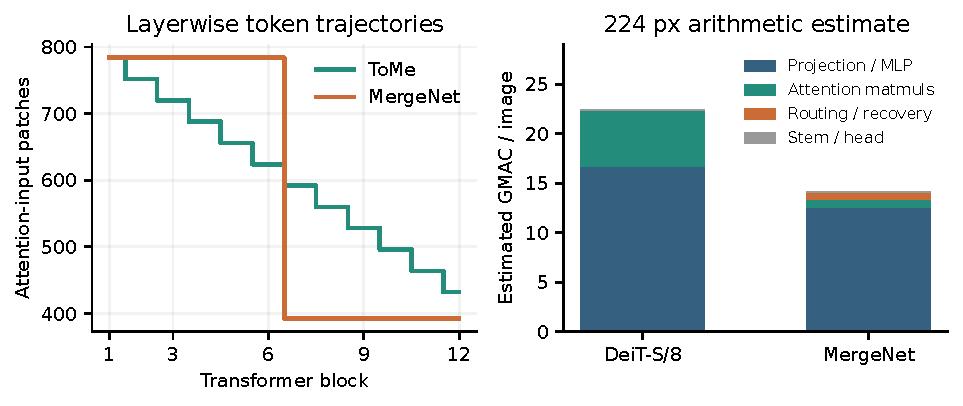
\includegraphics[width=\linewidth]{figures/cost_and_tokens.pdf}
\caption{Two code-derived views of cost. Left: the attention-input patch
trajectory at a final budget of 392; ToMe merges within blocks, while \mn{}
physically reduces the sequence between stages. ToMe's MLP inputs can be
shorter than its attention inputs. Right: analytic MAC components, with
non-arithmetic operations omitted from the count. Recovery is included in
the \mn{} routing/recovery component. These are not measured GPU profiles.}
\label{fig:cost}
\end{figure}

The guarded synthetic benchmark nevertheless measures \mn{} inference at
45.71\,ms per batch, versus 42.68\,ms for dense DeiT-S/8
(Table~\ref{tab:efficiency}). \mn{} takes 7.1\% more inference time and 3.5\%
more training-step time in this experiment. It also uses more peak allocated
memory. DeiT-S/16 is substantially faster, reinforcing that the accuracy gain
from retaining a finer input grid has a real execution cost.

\begin{table}[t]
\centering\footnotesize
\setlength{\tabcolsep}{4pt}
\begin{tabular}{lrrrrrr}
\toprule
Model & Params (M) & Train (ms) & Infer (ms) & IQR (ms) & Train GiB & Infer GiB \\
\midrule
DeiT-S/16 & 22.05 & 37.62 & 9.99 & 0.005 & 2.472 & 0.367 \\
DeiT-S/8 & 22.06 & 149.56 & 42.68 & 0.099 & 8.555 & 0.799 \\
MergeNet, $R=3$ & 23.10 & 154.87 & 45.71 & 0.073 & 10.071 & 1.125 \\
\bottomrule
\end{tabular}

\caption{September 5, 2026, 224-pixel batch-64 synthetic H20-3e benchmark, with random model
initialization and fp16 autocast. Train time includes forward, loss, backward
and AdamW update. Infer time is a forward-only median; the IQR column refers
to inference. Memory is peak \emph{allocated} GiB. These model-execution cells
are separate from the trained-checkpoint accuracy experiments.}
\label{tab:efficiency}
\end{table}

Several implementation properties offer plausible explanations. Full-grid
local MLPs and projections remain, sparse routing introduces indexed access
and reductions, the threshold operator performs sorting and cumulative
operations, and global recovery adds another attention operation. However,
the delivered decomposition uses CPU operator profiles and analytic byte
estimates. Its dispatch counts are not measured CUDA kernel-launch counts,
and its logical tensor traffic is not measured HBM traffic. We therefore do
not infer a proven memory-bandwidth bottleneck, a measured arithmetic
intensity, or an end-to-end speedup from a proposed kernel optimization.

At 384 pixels, the guarded batch-64 radius-3 benchmark measures 136.54\,ms
for \mn{} inference and 170.61\,ms for dense DeiT, a 20.0\% reduction in
batch time. A batch-128 run measures 262.02 versus 324.36\,ms, a 19.2\%
reduction; its training-step times are 889.76 versus 1135.48\,ms. Thus the
measured cost balance changes with resolution. These architecture benchmarks
use random initialization and remain distinct from checkpoint accuracy. A
later radius-5.143 latency sweep measures ToMe with proportional attention
\emph{disabled}, unlike the accuracy sweep. It also uses slightly different
achieved patch counts and retains token-counting hooks during timing.
Appendix~\ref{app:latency} reports these cells with their actual settings.
The available record does not support attaching the earlier accuracy scores
to these times or declaring that one method dominates the other on both axes.
A common harness must use the same attention policy, actual budget, checkpoint
identity, precision and hook-free timed path before making that claim.

\subsection{Trained-checkpoint joint evaluation: reserved frontier}
\label{sec:pending-frontier}
\pendingslot{P03}{Pair accuracy and timing from one verified configuration}{The
weights can remain on the collaborator's machine; return only permitted
evaluation records and figures.}

For each dense, MergeNet, ToMe and PiToMe cell, bind a checkpoint fingerprint
and state key to the same resolved arguments, resolution, preprocessing,
precision, batch composition and achieved patch budget. ToMe proportional
attention must agree between accuracy and timing. Count class tokens
separately, verify per-layer shapes, and remove hooks before timing.
Evaluate all 50,000 validation images. For the batch-dependent historical
selector, fix evaluation batches, ordering and distributed partitioning.

Measure on an otherwise idle device. Archive warmup/repetition counts,
synchronized CUDA-event samples, medians and IQRs. Report allocated and
reserved memory separately, and specify whether latency includes data loading.
Synthetic-input measurements remain labeled as model-execution timings.
Do not join the old accuracy sweep to another random-weight configuration.

\begin{table}[htbp]\centering\small
\begin{tabular}{lrrrrr}\toprule
Method & Patches & EMA top-1 & Median ms & IQR ms & Allocated GiB\\\midrule
Dense DeiT-S/8 & \pendingvalue & \pendingvalue & \pendingvalue & \pendingvalue & \pendingvalue\\
MergeNet & \pendingvalue & \pendingvalue & \pendingvalue & \pendingvalue & \pendingvalue\\
ToMe & \pendingvalue & \pendingvalue & \pendingvalue & \pendingvalue & \pendingvalue\\
PiToMe & \pendingvalue & \pendingvalue & \pendingvalue & \pendingvalue & \pendingvalue\\
\bottomrule\end{tabular}
\caption{Reserved trained-checkpoint joint cells [P03]. Repeat this block
for each resolution/budget and attach device, batch, state key and attention
policy. All numerical fields remain unfilled.}
\label{tab:pending-frontier}\end{table}
\begin{figure}[htbp]\centering
\pendingfigure{P03: measured accuracy versus batch latency at 224 and 384 pixels}{3.5cm}
\caption{Reserved joint comparison [P03]. No dominance ordering is assumed.}
\label{fig:pending-frontier}\end{figure}
\pendingtext

\subsection{ImageNet selector transfer: reserved experiment}
\label{sec:pending-selector}
\pendingslot{P05}{Separate batch invariance from learning behavior}{Completed
CIFAR runs do not determine ImageNet accuracy after a selector change.}

Hold selected images fixed while replacing only their batch companions.
Compare exact repeats, original selection and rowwise selection; export logit
differences, changed classes, selection-mass errors and finite-gradient checks.
A learning claim additionally requires matched ImageNet training. Changing
the operator in old weights is an inference intervention. The rowwise
implementation changes normalization and threshold solution together;
attributing an effect to one component needs additional factorial controls.
Generalizing the issue to other implementations requires their own audits.

\begin{table}[htbp]\centering\small
\begin{tabular}{lrrrr}\toprule
Condition & Top-1 & Max logit change & Changed classes & Finite checks\\\midrule
Original selector, old weights & \pendingvalue & \pendingvalue & \pendingvalue & \pendingvalue\\
Rowwise intervention, same weights & \pendingvalue & \pendingvalue & \pendingvalue & \pendingvalue\\
Matched rowwise training & \pendingvalue & \pendingvalue & \pendingvalue & \pendingvalue\\
\bottomrule\end{tabular}
\caption{Reserved ImageNet selector tests [P05]. Image population, batches,
seeds and state identities accompany each distinct experimental condition.}
\label{tab:pending-selector}\end{table}
\pendingtext

\subsection{Execution-cost attribution: reserved profile}
\label{sec:pending-profile}
\pendingslot{P08}{Measure device activity and complete training steps}{Needed
for a specific bottleneck explanation or training-speed claim.}

Profile local attention/MLPs, selection, transport, gather, recovery and
latent blocks on one fixed software stack. Device operator times may overlap
and must not be assumed additive. HBM bandwidth claims require device counters,
not logical tensor sizes. Compare layouts with identical inputs, loss,
backward, optimizer and AMP policy; report actual updates and skipped steps.
Long-run accuracy or stability needs separate matched training. The existing
approximate 5\% inference gain does not fill these training cells.

\begin{table}[htbp]\centering\small
\begin{tabular}{lrrrr}\toprule
Implementation & Step median ms & IQR ms & Allocated GiB & Actual updates\\\midrule
Original layout & \pendingvalue & \pendingvalue & \pendingvalue & \pendingvalue\\
Layout variant & \pendingvalue & \pendingvalue & \pendingvalue & \pendingvalue\\
\bottomrule\end{tabular}
\caption{Reserved complete-step timing [P08]. Per-region device profiles
and any long-run checks are separate evidence.}
\label{tab:pending-profile}\end{table}
\pendingtext

